% {{{ LaTeX Preamble
\documentclass{article}

\usepackage{hyperref}

\usepackage{listings}

\usepackage{amsthm}
\theoremstyle{definition}
\newtheorem{example}{Example}[section]

\newif\ifusenatbib
\usenatbibtrue
%\usenatbibfalse

\ifusenatbib
\usepackage{natbib}
\bibliographystyle{myabstract}
\usepackage{bibentry}
\nobibliography*
\else
\usepackage[style=authoryear-comp,natbib=true]{biblatex}
\bibliography{biblio}
\fi

\newcommand{\htmlanchorstart}[1]{%
	\ifx\HCode\Undef%
		\empty%
	\else%
		\HCode{<a id="#1"></a>}%
	\fi%
}
\newcommand{\htmlanchorend}[1]{%
	\ifx\HCode\Undef%
		\empty%
	\else%
		\HCode{<a href="\##1">&para;</a>}%
	\fi%
}
\newcommand{\htmlspantitle}[2]{%
	\ifx\HCode\Undef%
		#1
	\else%
		\HCode{<span title="#2">#1</span>}%
	\fi%
}

% {{{ Print article title
%%%%%%%%%%%%%%%%%%%%%%%%%%%%%%%%%%%%%%%%%%%%%%%%%%
\usepackage{usebib}
\newbibfield{abstract}
%% prints out the info for a citation key:
%%     \printarticle{Author00}
\newcommand{\printarticle}[1]{\citeauthor{#1}, ``\usebibentry{#1}{title}'' (\usebibentry{#1}{year})}
\newcommand{\printarticlespanabstract}[1]{\htmlspantitle{\usebibentry{#1}{title}}{\usebibentry{#1}{abstract}}}
\newcommand{\printarticletitleonly}[1]{\usebibentry{#1}{title}}
\newcommand{\paracitecite}[1]{\printarticletitleonly{#1}~\citet{#1}}
\newcommand{\paracite}[1]{\paragraph{\htmlanchorstart{bibentry:#1}\paracitecite{#1}}\label{bibentry:#1}\htmlanchorend{bibentry:#1}}
% \bibentry{#1}
%%%%%%%%%%%%%%%%%%%%%%%%%%%%%%%%%%%%%%%%%%%%%%%%%% }}}

\bibinput{biblio}

\def\printindex{}

\usepackage{graphicx}
\usepackage{tikz}
\usetikzlibrary{arrows,positioning}

% {{{ External TikZ
% <http://tex.stackexchange.com/questions/40135/htlatex-and-tikz-creates-sometimes-incorrect-svgs>
% <http://tex.stackexchange.com/questions/158551/using-htlatex-with-tikz-dependency>
\usetikzlibrary{external}
\tikzset{
	png copy/.style={
		external/system call={
				pdflatex \tikzexternalcheckshellescape -halt-on-error -interaction=batchmode -jobname "\image" "\texsource";
				mutool draw -r 300 -o "\image.png" "\image.pdf";
				mogrify -transparent white "\image.png"
		}
	}
}
		%convert -density 300 -transparent white "\image.pdf" "\image.png"
\tikzset{png copy}
\makeatletter
\@ifpackageloaded{tex4ht}{
	\tikzexternalize[mode=only graphics]
	\tikzset{png export/.style={/pgf/images/external info,/pgf/images/include external/.code={\includegraphics{##1.png}}}}
%[width=\pgfexternalwidth,height=\pgfexternalheight]
	\tikzset{png export}
}{
	\tikzexternalize
	\tikzset{pdf export/.style={/pgf/images/external info,/pgf/images/include external/.code={\includegraphics{##1.pdf}}}}
%[width=\pgfexternalwidth,height=\pgfexternalheight]
	\tikzset{pdf export}
}
% }}}


% }}}
\begin{document}


% {{{ Configuration
% {{{ configure graphics for TeX4ht
\ifx\HCode\Undef \empty \else%
\makeatletter

% PDF page graphics {{{
\define@key{Gin}{page}[1]{\def\Gin@page{#1}}
\makeatother
	\Configure{graphics*}{pdf}
			{\Needs{"mutool draw -r 300 -o \jobname\arabic{texforhtimagecounter}y.png \csname input@path\endcsname/\csname Gin@base\endcsname.pdf \csname Gin@page\endcsname"}%
				\Picture[pict]{\jobname\arabic{texforhtimagecounter}y.png
				\space style="width: \space  \csname Gin@html@width\endcsname \space !important;
				\space float: \csname Gin@html@float\endcsname;
				\space clear: both;
				"}%
			\stepcounter{texforhtimagecounter}%
				\special{t4ht+@File: \csname Gin@base\endcsname.png}
				}

			%{\Needs{"convert \csname Gin@base\endcsname.pdf
				%\csname Gin@base\endcsname.png"}%
% }}}


% Configure graphics for PNG, JPEG {{{
% From <http://tex.stackexchange.com/questions/46156/pdf-image-files-and-htlatex>
	\DeclareGraphicsExtensions{.png,.jpg,.jpeg}
	\newcounter{texforhtimagecounter}
	\newcommand{\ConfigureGraphicsDirect}[3]{%
		\Configure{graphics*}
				{#1}
				{\Needs{"#3 \csname Gin@base\endcsname.#1
					\jobname\arabic{texforhtimagecounter}y.#2"}%
					\Picture[pict]{\jobname\arabic{texforhtimagecounter}y.#2}%
					\stepcounter{texforhtimagecounter}%
				}%
	}
	%\ConfigureGraphicsDirect{pdf}{png}{convert -density 300}%
	\ConfigureGraphicsDirect{png}{png}{cp}%
	\ConfigureGraphicsDirect{jpg}{jpg}{cp}%
	\ConfigureGraphicsDirect{jpeg}{jpg}{cp}%
\fi
% }}}
% }}}

\section{Bret Victor}

\begin{itemize}
\item \url{http://worrydream.com/MediaForThinkingTheUnthinkable/note.html}
\item \url{http://worrydream.com/MediaForThinkingTheUnthinkable/}
\item \url{http://worrydream.com/MagicInk/}
\item \url{http://worrydream.com/TheHumaneRepresentationOfThought/note.html}
\end{itemize}

\section{Alan Kay}

\url{https://www.youtube.com/watch?v=YyIQKBzIuBY}, \href{http://www.tele-task.de/archive/video/flash/14029/}{HPI}

\section{Design of electronic books}

\paracite{marshall2009-reading}

\paracite{pearson2013-digital-reading}

\section{Software engineering}

\paracite{rosenberg2008-dreaming-code}

\section{Workflow}

In \href{http://ahiddendiscourse.com/2013/02/17/the-cognitive-basis-for-academic-workflows/}{The cognitive basis for academic workflows},
Lisa D. Harper looks at sensemaking models as a way to understand academic
workflows.

\section{Scene graphs}

\paracite{tavenrath2016}

\begin{itemize}
\item dynamic scene graph: many updates
\item extract just transform nodes to a transform tree
\end{itemize}


\[ T_{2,world} = T_{2,local} \cdot T_{0,local} \cdot T^{*}_{local} \]

The world matrix is used for shader, culling, bounding box, collision
detection.

\begin{figure}
\tikzsetnextfilename{tavenrath2016-fig1}
% vim: ft=tex
\usetikzlibrary{arrows,positioning}
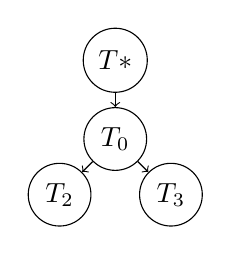
\begin{tikzpicture}[
		every node/.style={draw,circle}
	]
	\node                     (Tst) {$T*$} ;
	\node [below of=Tst]      (T0) {$T_0$} ;
	\node [below left of=T0]  (T2) {$T_2$} ;
	\node [below right of=T0] (T3) {$T_3$} ;

	\draw [->] (Tst) -- (T0) ;
	\draw [->] (T0)  -- (T2) ;
	\draw [->] (T0)  -- (T3) ;
\end{tikzpicture}

\caption{Example tree}
\end{figure}

\paracite{worister2013lazy}

\begin{itemize}
\item \fbox{scene graph} creates \fbox{dependency graph}
\item \fbox{program} updates \fbox{scene graph} updates$*$
	\fbox{dependency graph} \\
	$*$ but only parts that are visible are updated
\end{itemize}

\paragraph{Update algorithm}

\paracite{reps1983incremental}

\paracite{hudson1991incremental}

They use a semantic scene graph as in
\paracitecite{tobler2011separating} --- traversal cost is high ---
caching eliminates this cost.

caching however occurs an overhead (see Table 1 of paper) at
startup time

need to benchmark the number of draw calls to see when it will pay
off: \( \uparrow \) draw calls, \(\downarrow\) frame rate.

can be parallelised


\paracite{tobler2011separating}

semantic graph is used to keep application state inside of graph

application acts like a compiler

semantic scene graph \( \rightarrow \) rendering scene graph

a single semantic scene graph node can build many intermediate
rendering scene graph nodes that differ based on rendering backend

applicator nodes are trees as well

transformation
\begin{itemize}
\item children: transformation matrices
\item aggregator: matrix multiplication
\end{itemize}

LOD node: returns a different scene graph based on level

multiple-view has both:
\begin{itemize}
\item shared data
\item private data
\end{itemize}
for
\begin{itemize}
\item traversal cache
\item traversal state
\end{itemize}

editing of semantic nodes
\begin{itemize}
\item back references
\item a little unclear why have 2 rendering scene graphs
  \begin{itemize}
  \item render normal
		\begin{verbatim}
		      ------
		      |    |
		      ------
		\end{verbatim}
	\item edit handles
		\begin{verbatim}
		      o    o
		            
		      o    o
		\end{verbatim}
  \item render w/ edit handles
		\begin{verbatim}
		      o----o
		      |    |
		      o----o
		\end{verbatim}
  \end{itemize}
\end{itemize}

rendering scene graph is cached by creating scene graph forest


\paracite{zeleznik2000scene}

networking


\subsection*{OpenSceneGraph}

TODO

\section{Attribute grammars}

Attribute grammars were first introduced by Knuth. They consist of
a normal grammar, but augmented with attributes. Attributes are
the results of calculations based on the values and attributes of
nodes in the parse tree.~\cite{knuth1968semantics}.

One issue with attributes grammars is determining the order of
evaluation. One naive approach is to use a topological sort based
on the dependency graph of the attributes.

\begin{example}
Example: Attribute grammar for summing values in list. Taken
from~\cite{steinlechner2019attrgrammars}.

Data structure
\begin{lstlisting}
interface List { }
class Cons : List {
	Int Value;
	List Rest;
}
class Nil : List { }
\end{lstlisting}

Attribute grammar (UUAGC syntax)
\begin{lstlisting}
syn SEM List
| Nil  this.Sum = 0
| Cons this.Sum = this.Value + this.Rest.Sum
\end{lstlisting}
\end{example}

In this example, the attribute grammar defines a \emph{synthesised
attribute} \texttt{Sum}. The order of evaluation is bottom-up and
since this grammar only uses a synthesised attribute, it is an
\emph{S-attributed grammar}.

There are also special classes of attribute grammars than can be
evaluated in a single pass during parsing despite having both
synthesised attributes and \emph{inherited attributes}.

For a synthesised attribute \(\alpha\) and production \( S \to ABC
\) the semantic function for \(S.\alpha\) can depend on attributes
from \(A\), \(B\), or \(C\).

For the inherited attribute \(\beta\) on the same production,
\(B.\beta\) can depend on attributes from \(S\), \(A\), or \(C\)
(every other symbol).

However, to evaluate a general class of attribute grammars, a
specific traversal would be needed for each attribute grammar
depending on the dependencies for the semantic functions. There
existed algorithms that can take a specific attribute grammar and
compute a traversal function for an attribute. Some of these are
implemented in the for of a code generating compiler (e.g., UUAGC,
JastAdd). UUAGC which uses a version of
the~\cite{kennedy1976automatic}) algorithm that is described
in~\cite{bransen2012kennedy}.

These algorithms are often used in an ahead of time compiler in
order to generate a static tree-walker evaluator. However, in some
applications, an online version may be useful for dynamic editing
of values on the trees or changes to the tree structure itself
(e.g., a language editor). This merges the work in attribute
grammars with work in incremental
computing~\cite{reps1983incremental,ramalingam1993categorized}.

In order to use attribute grammars in a way that they can be
composable (in FP, AGs can be used to define catamorphisms
compositionally) and easy to write, there has been work on making
embedded DSLs for AG definitions \cite{sloane2010pure}.


\section{Incremental computing}

\section{Self-adjusting computation}


%\nocite{*}
\ifusenatbib
	\bibliography{biblio}
\else
	\printbibliography
\fi

\end{document}
